\documentclass{standalone}
\usepackage{pgfplots}
\usetikzlibrary{decorations.markings}
\usepackage{physics}
\begin{document}
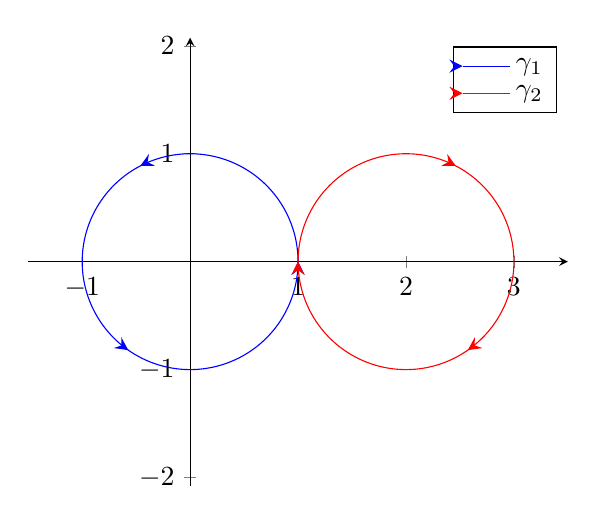
\begin{tikzpicture}[>=latex]
\begin{axis}[
	axis lines = center,
	axis equal,
	xmin = -1.5,
	xmax = 3.5,
	ymin = -1.5,
	ymax = 1.5
	]
	\addplot[
		domain = 0:360,
		samples = 1000,
		color = blue,
		decoration={
			markings,
			mark = between positions 0 and .9 step 8em with {\arrow [scale=1.5]{stealth}}
			},
		postaction = decorate
		]
		({cos(x)},{sin(x)});
	\addplot[
		domain = 180:540,
		samples = 1000,
		color = red,
		decoration={
			markings,
			mark = between positions 0 and .9 step 8em with {\arrow [scale=1.5]{stealth}}
		},
		postaction = decorate
		]
		({2 + cos(x)},{-sin(x)});
	\legend{\(\gamma_1\),\(\gamma_2\)}
\end{axis}
\end{tikzpicture}
\end{document}